\documentclass{report}

\usepackage[utf8]{inputenc}
\usepackage[T1]{fontenc}
\usepackage[francais]{babel}
\usepackage{url}
\usepackage{color}
\usepackage{verbatim}
\usepackage{amsmath,amssymb,amsfonts}
\usepackage{graphicx}
\usepackage[french]{algorithm2e}

\title{Introduction aux Réseaux : TP1}
\author{Line \bsc{POUVARET}, Mickaël \bsc{TURNEL}}
\date{2015-2016}


\begin{document}

\maketitle

\chapter*{Compte-Rendu de TP}
\section*{2.1 	Mise en place du réseau}
	\subsection*{2.1.2	Configuration des machines}

\subsubsection*{Configuration manuelle}
Nous avons choisi comme adresse IP Internet 134.134.134.X, X étant le numéro de machine allant de 1 à 4.
Pour chaque machine, nous avons exécuté la commande : ifconfig em0 134.134.134.X up
Si on exécute à nouveau ifconfig sur chaque machine, on constate bien que nous obtenons la bonne adresse configurée pour inet et que status est à active.

Nous avons modifié le fichier /etc/hosts de chaque machine de sorte à avoir :
134.134.134.1 M1
134.134.134.2 M2
134.134.134.3 M3
134.134.134.4 M4

	\subsection*{2.1.3	Contrôle du réseau}

\subsubsection*{Utilisation du ping}
Nous avons effectué une commande ping sur chaque machine vers les trois autres machines du réseau. (ex sur M2: ping M1, ping M3, ping M4)\\
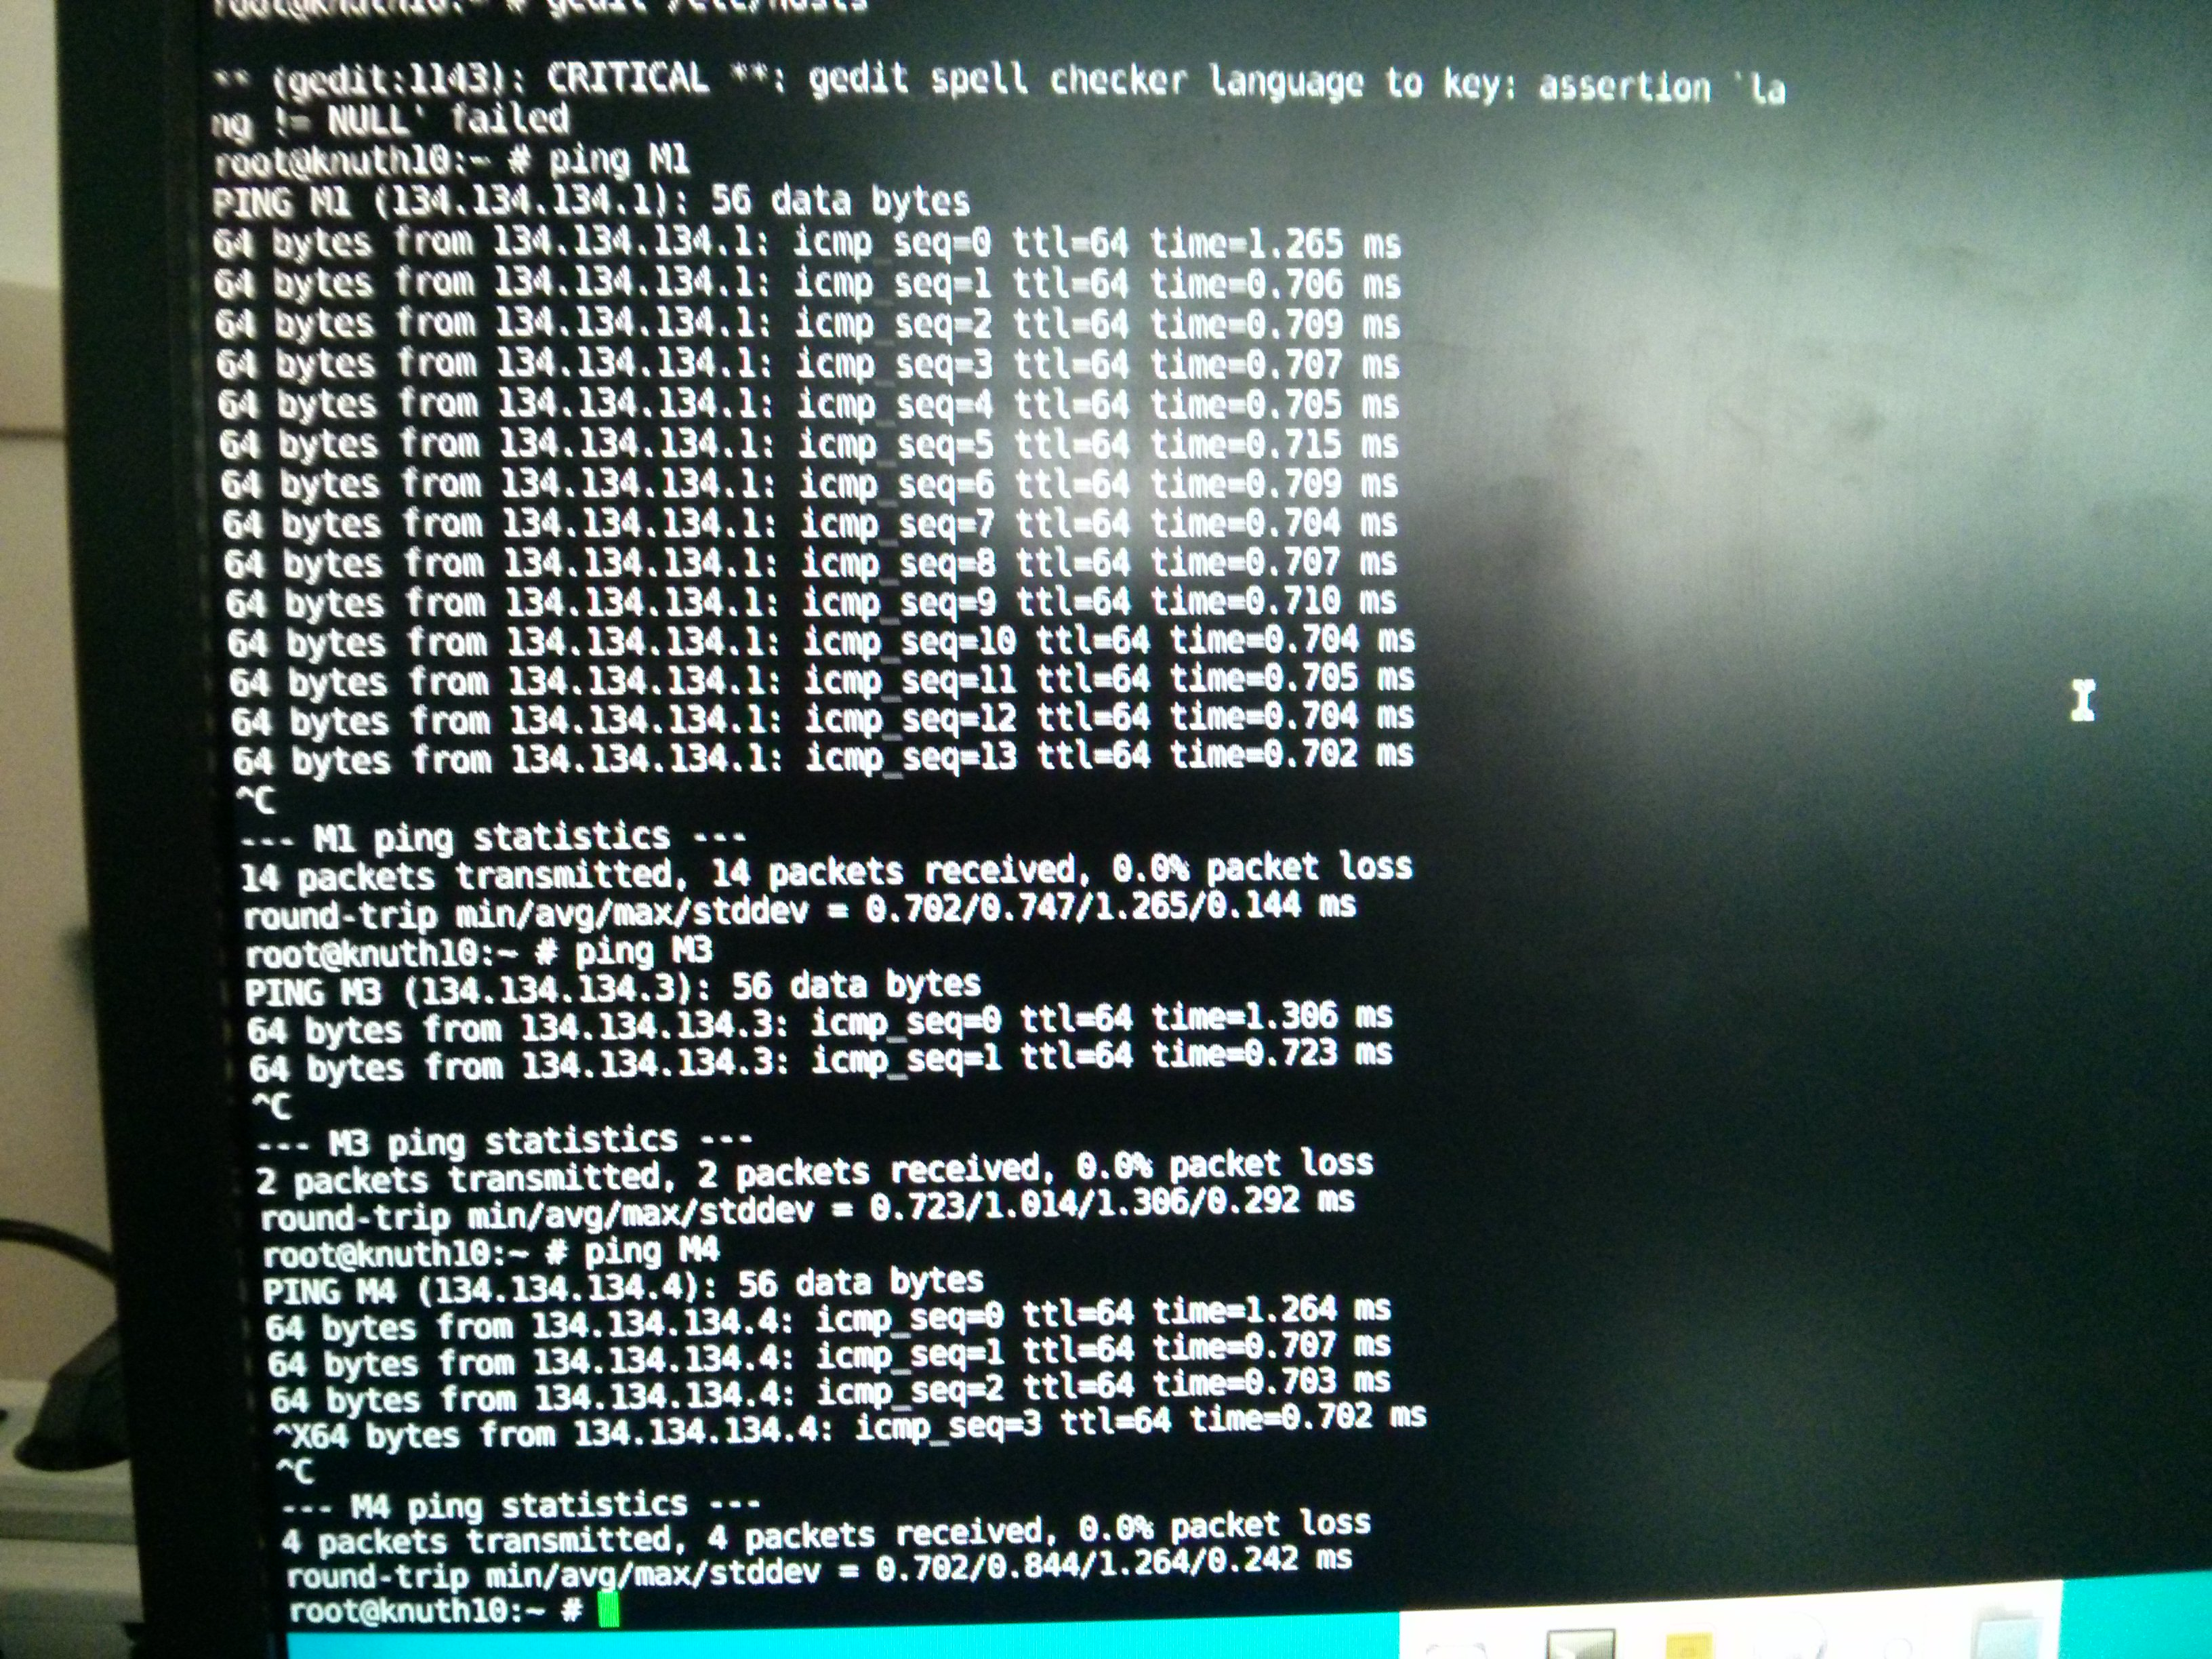
\includegraphics[width=12cm]{screen1.jpg}


\subsubsection*{Procédure de login sur une machine distante}
Nous avons utilisé l'application telnet pour que la machine M2 communique avec M4 en exécutant la commande suivante : telnet -y M4
En exécutant ifconfig (toujours dans l'application telnet) sur M2, on remarque que l'adresse inet est bien 134.134.134.4 (c'est à dire l'adresse Internet de M4)\\
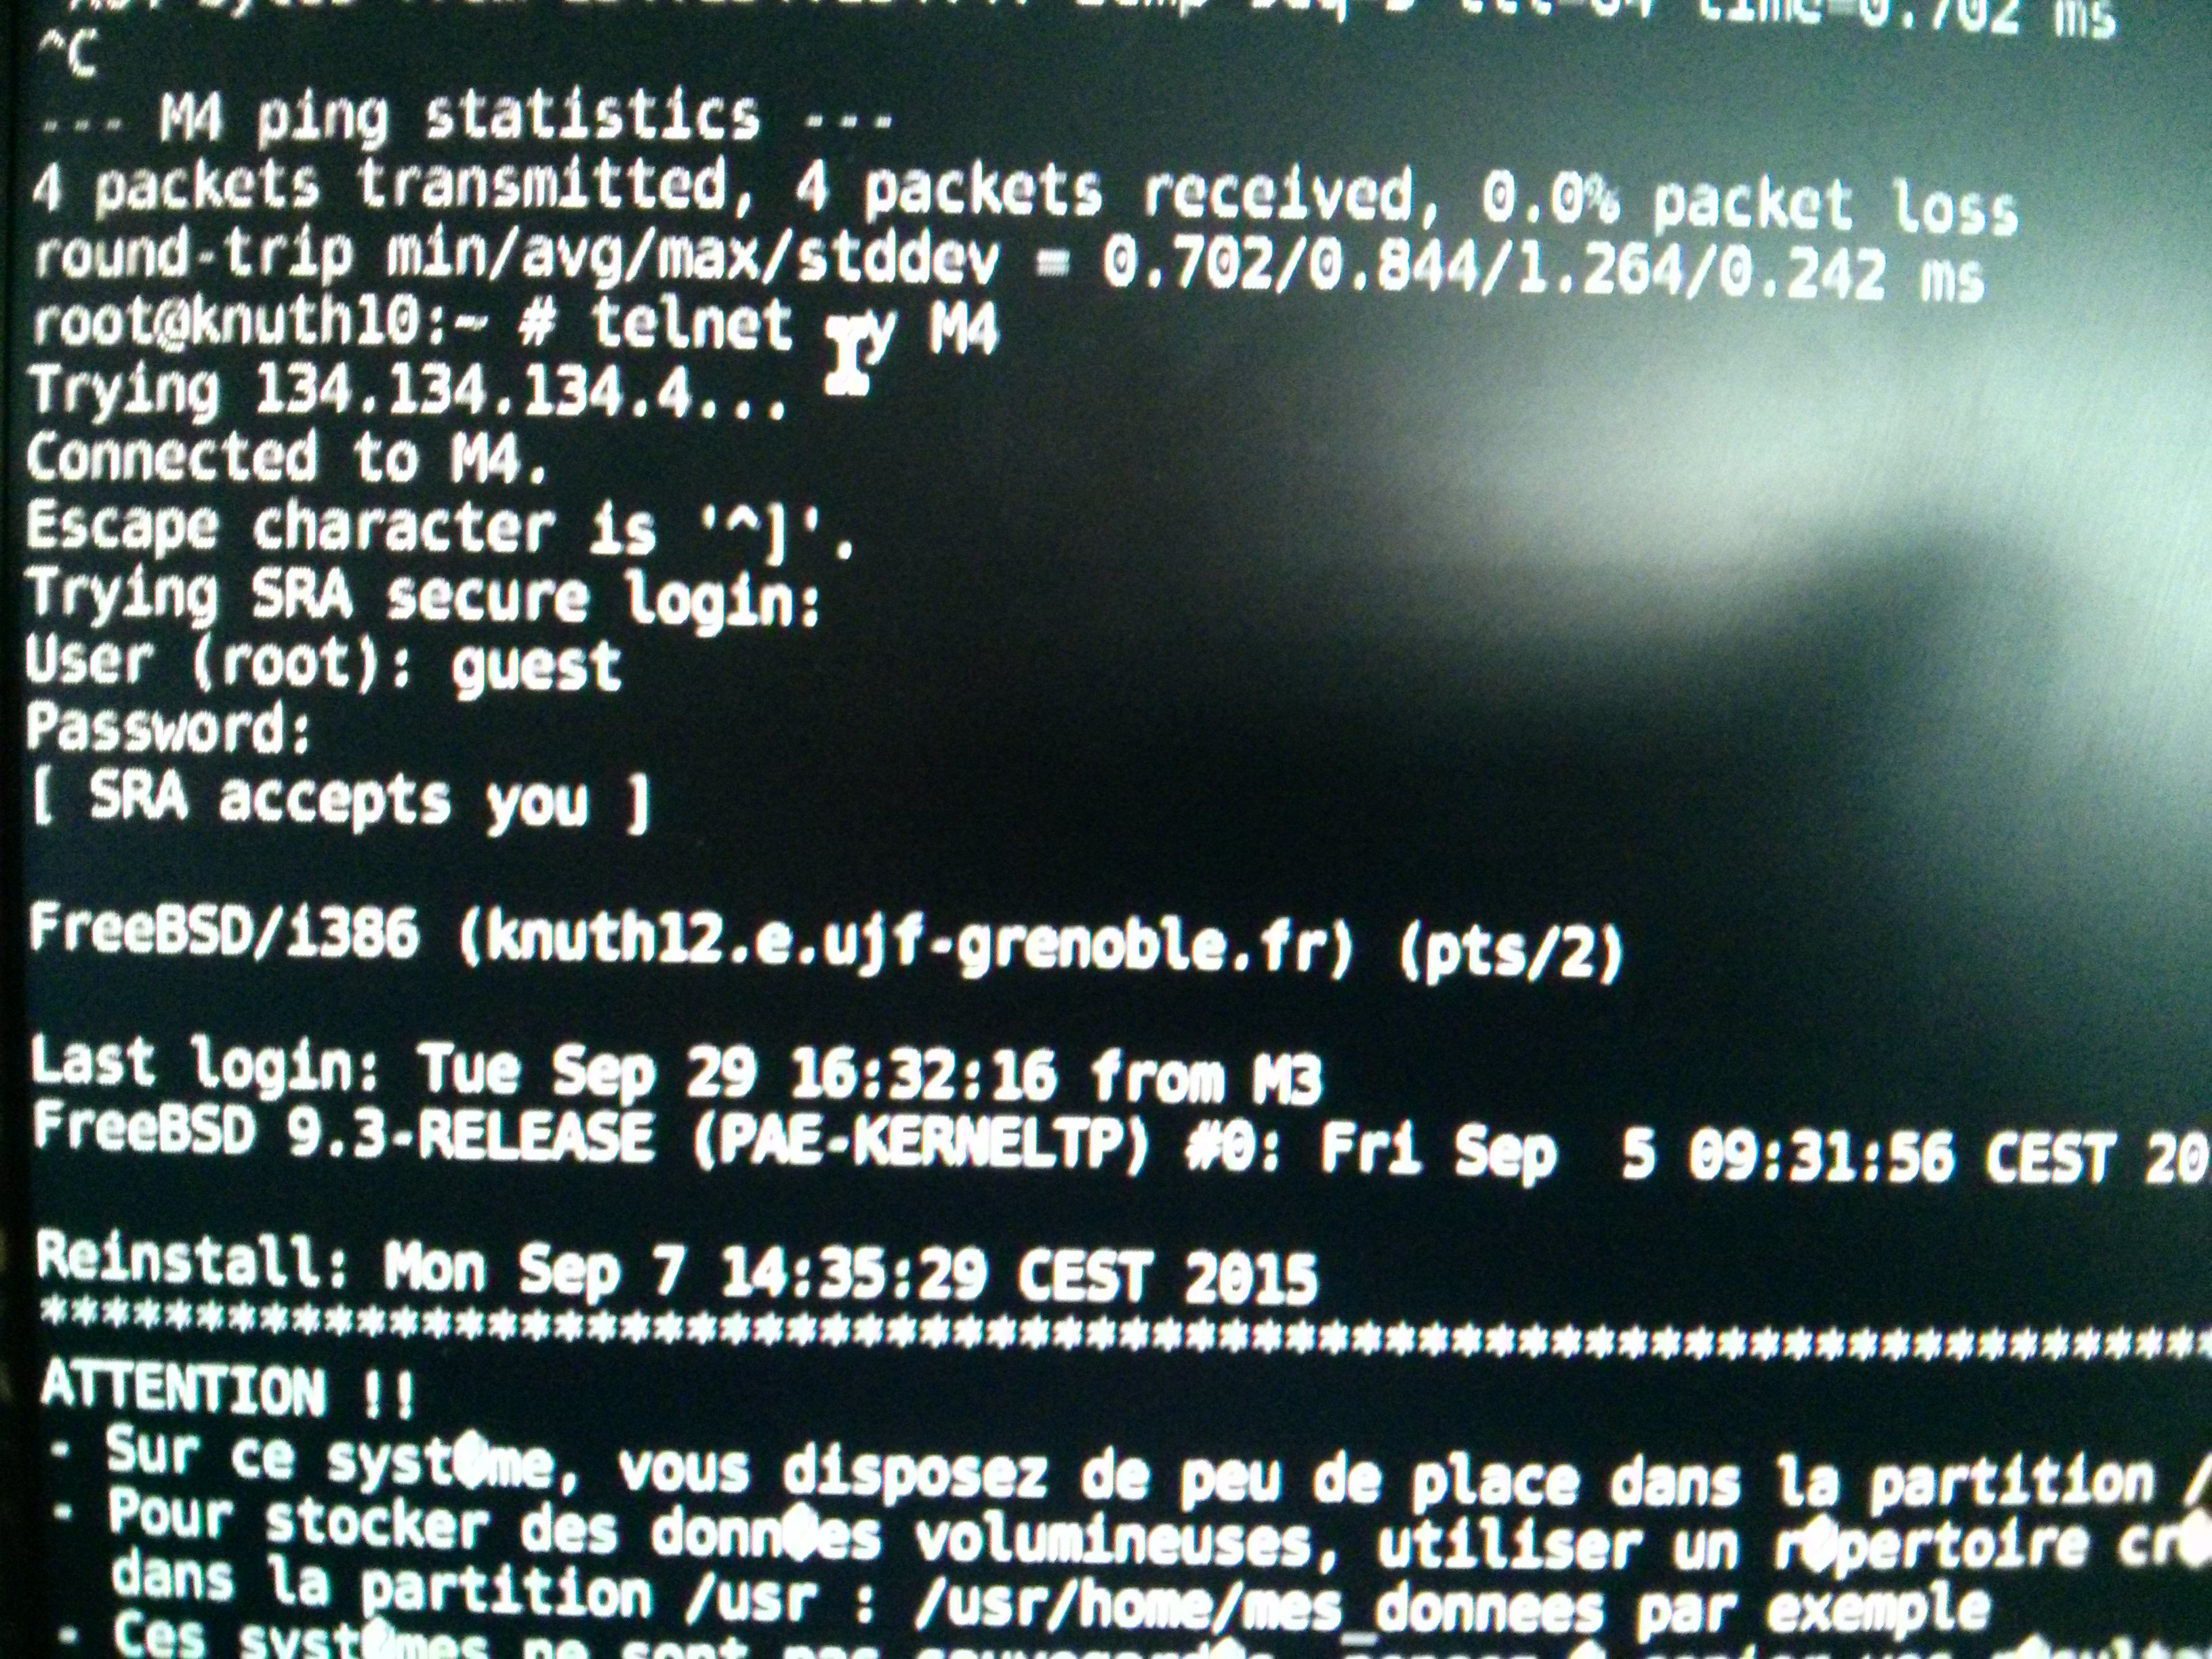
\includegraphics[width=10cm]{screen2.jpg}
\\
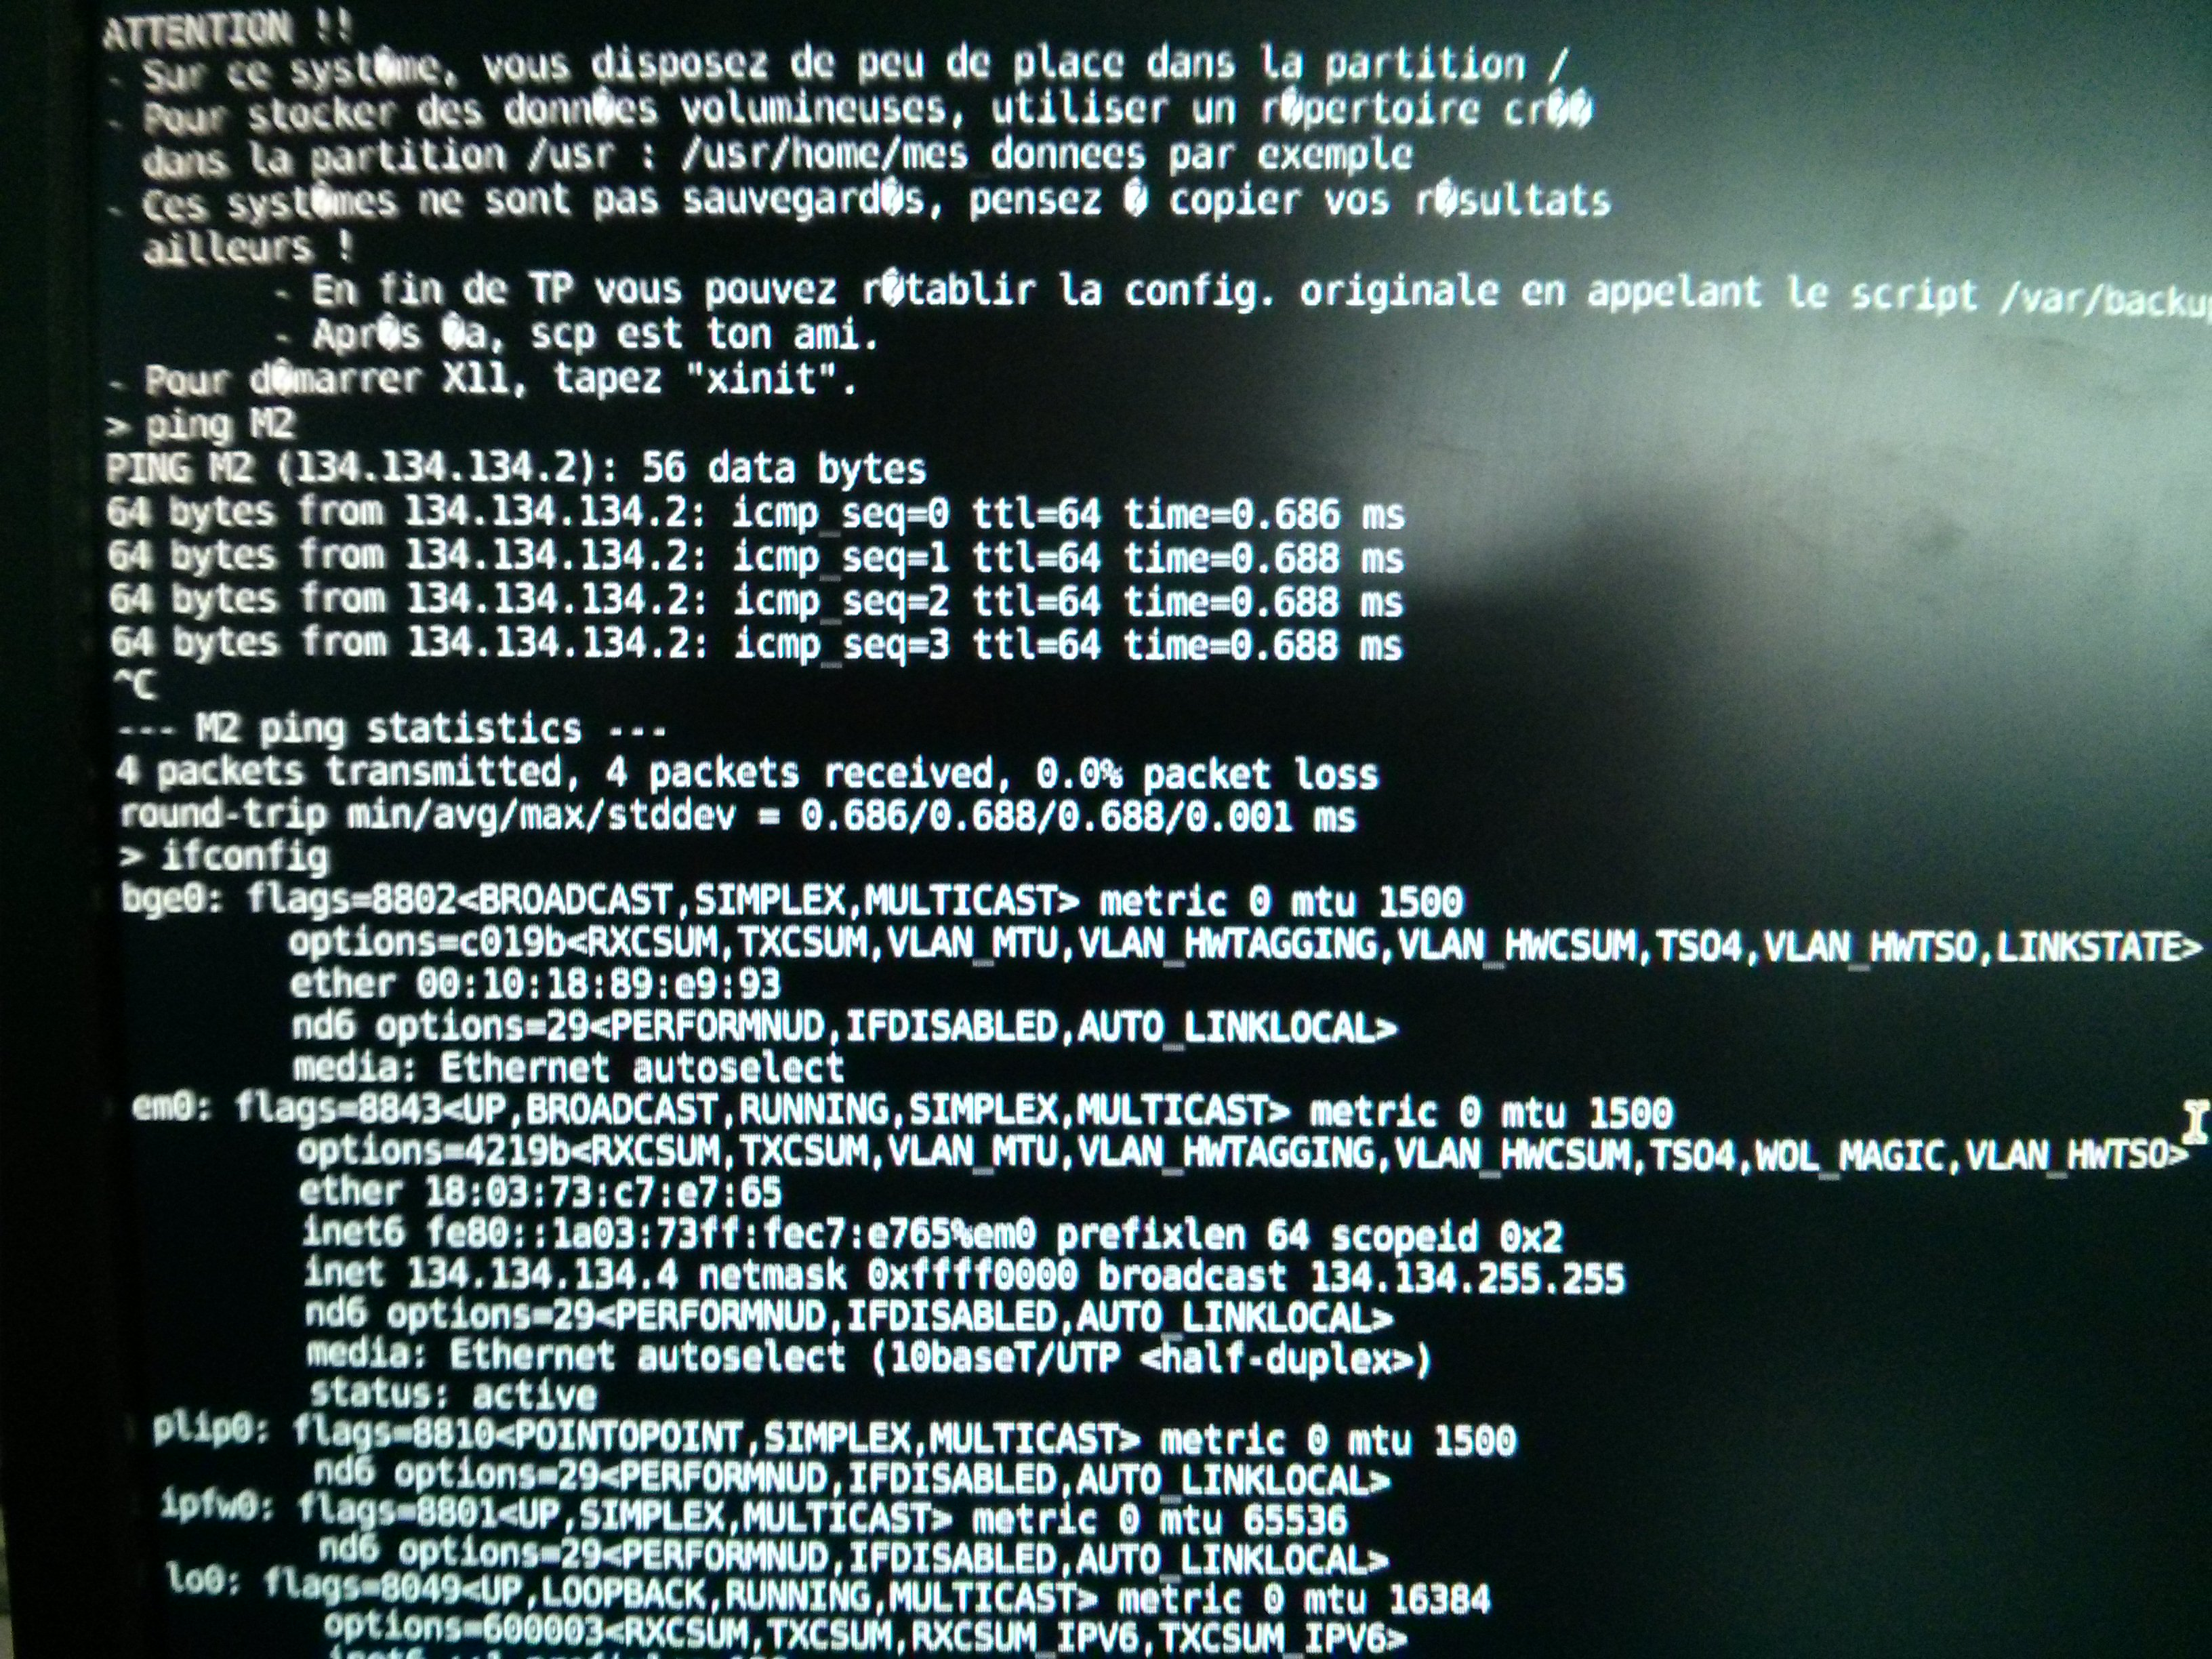
\includegraphics[width=12cm]{screen3.jpg}

\section*{2.2 Observation de l'activité du réseau}

Nous avons lancé Wireshark sur M2 (134.134.134.2) et exécuté une commande ping de M1 vers M3.\\

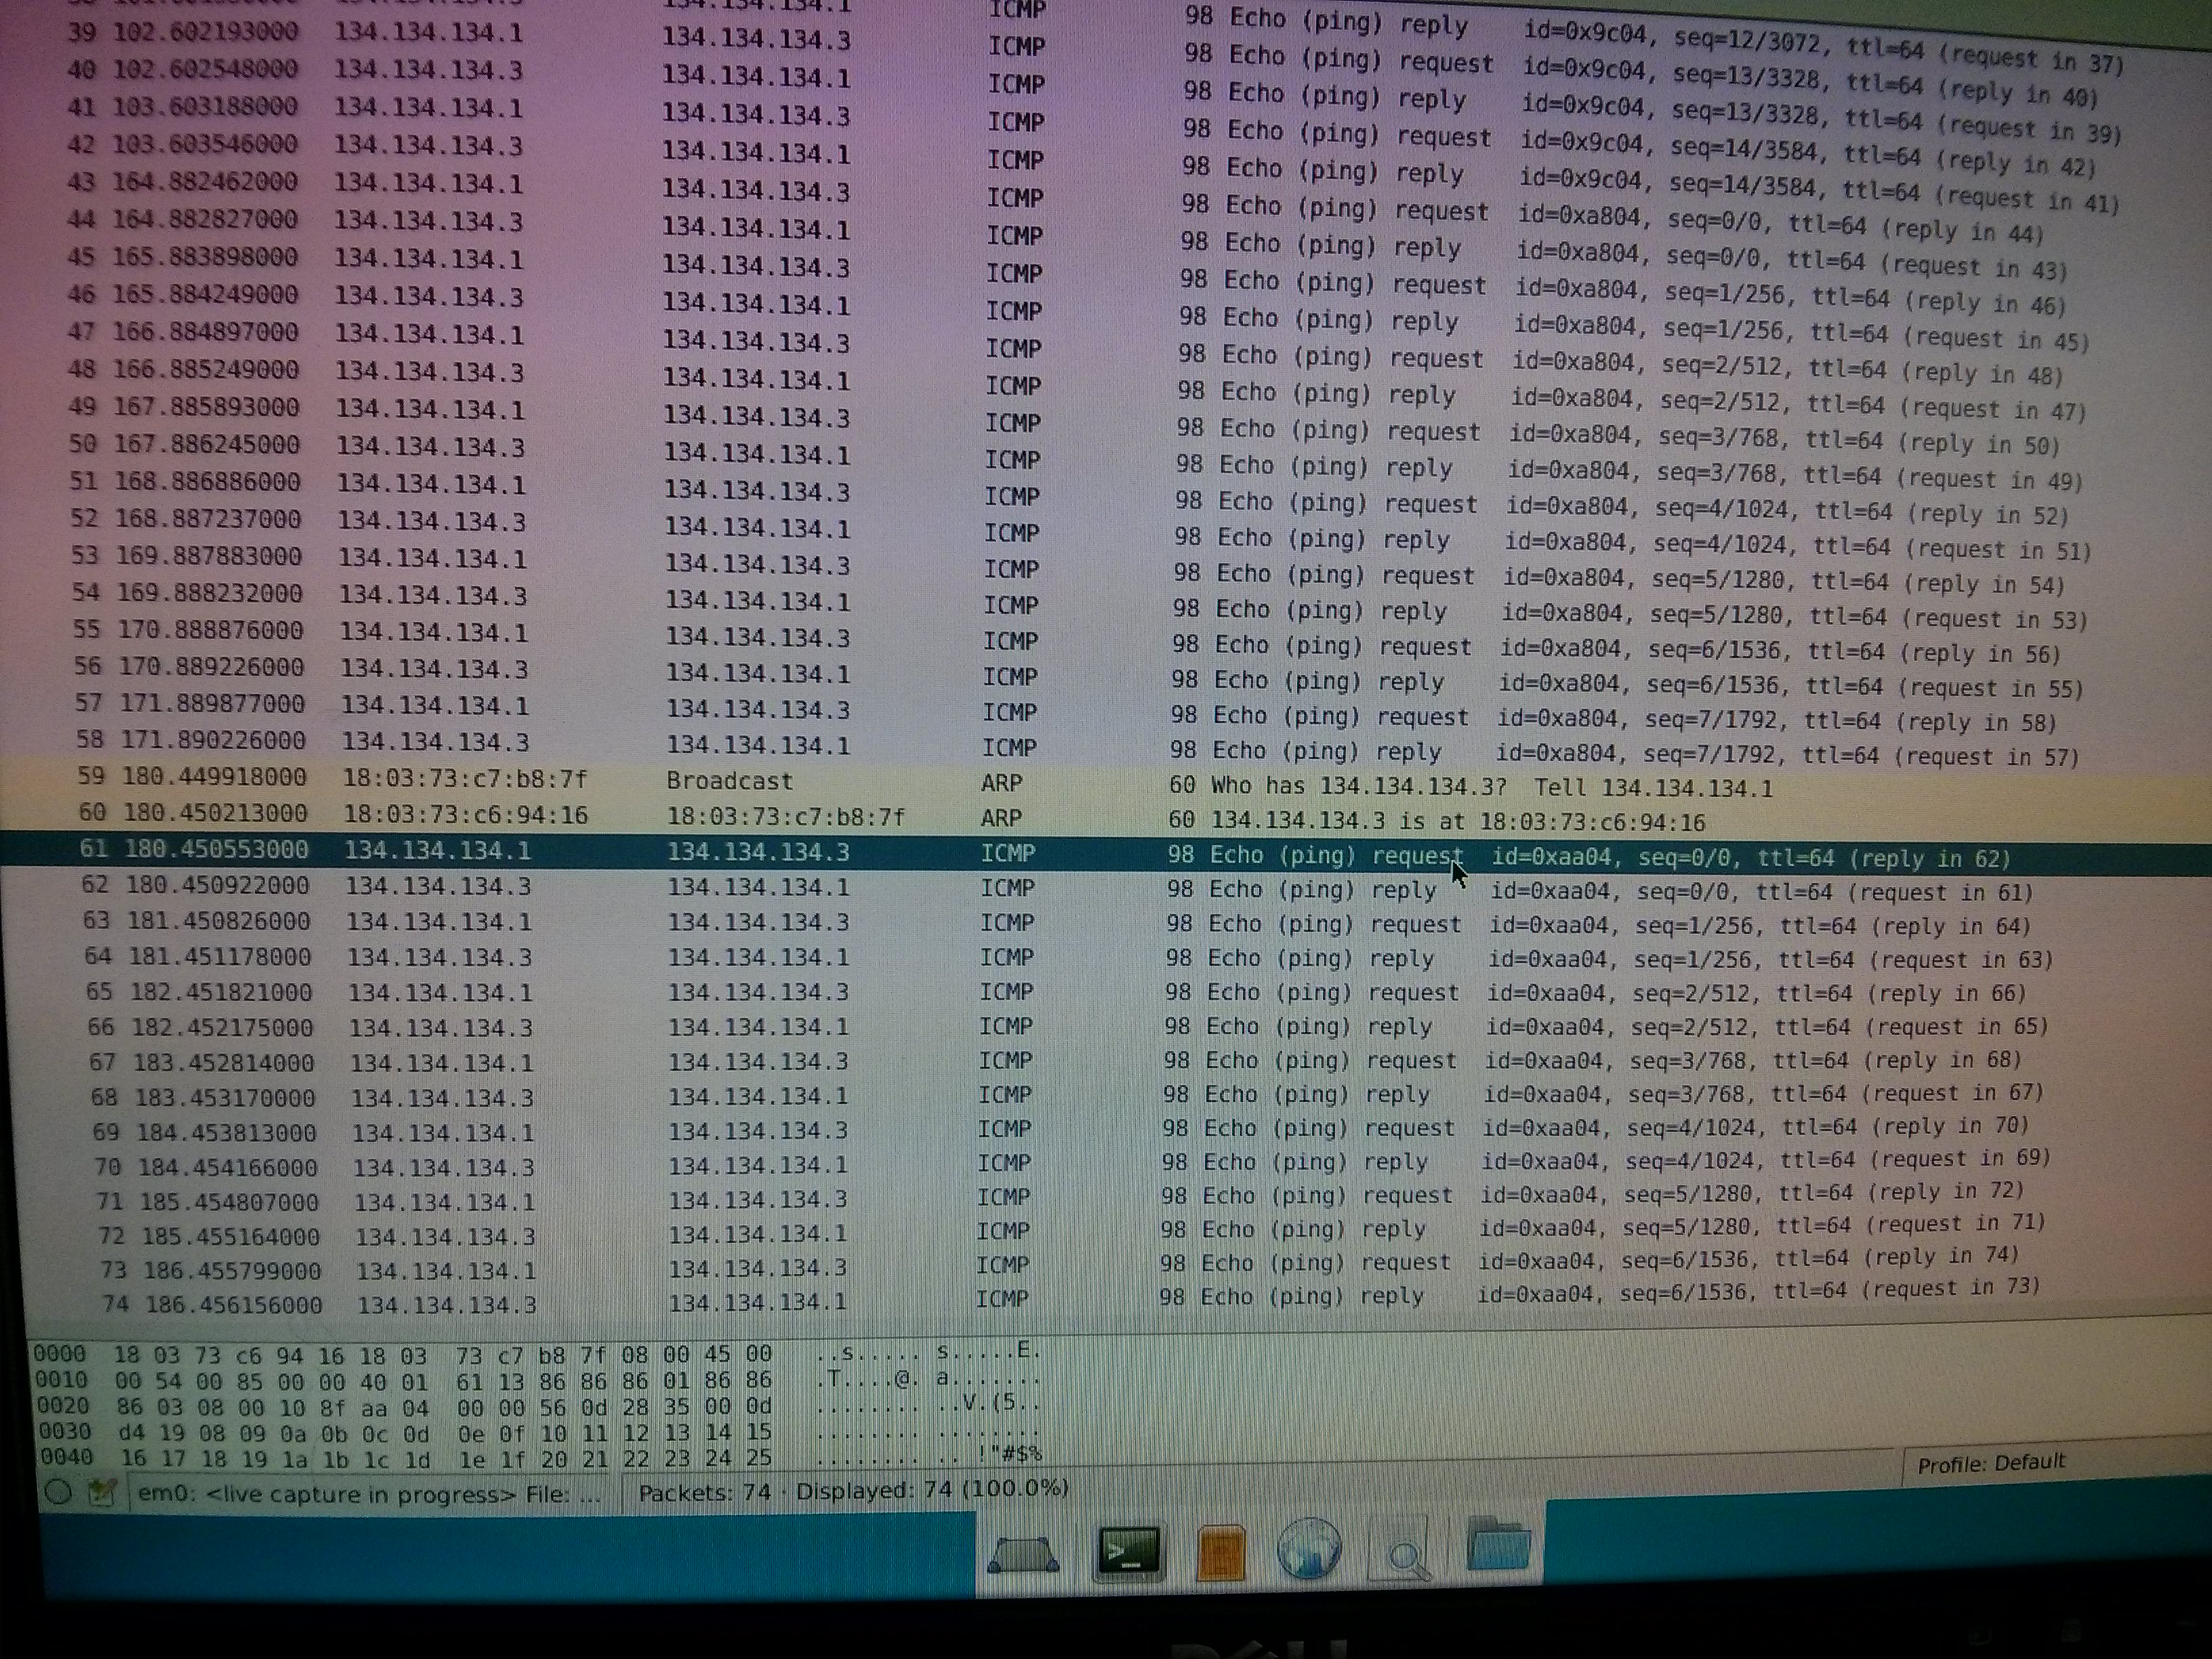
\includegraphics[width=12cm]{screen4.jpg}\\

\subsection*{Observation de la commande ping}

\begin{itemize}\renewcommand{\labelitemi}{$\bullet$}
\item Ping envoie une requête à la machine M3 (dans notre exemple), la source de la requête a l'adresse 134.134.134.1 et le destinataire a l'adresse \\134.134.134.3 et la machine M3 envoie une réponse à M1 (destinataire vers la source).
Ici les paquets envoyés sont visibles par toutes les machines (car M2 peut observer tous les paquets qui transitent par le hub) mais seulement le destinataire du ping (M3) répond (en envoyant un paquet).

\item Quand la source du ping ne connait pas l'adresse Ethernet du destinataire (d'adresse Internet connue 134.134.134.3), il envoie à tout le monde un paquet de type ARP afin de demander aux autres machines quelle est l'adresse Ethernet de 134.134.134.3 et la machine concernée répond à la source en lui donnant son adresse Ethernet via un paquet de type ARP.

\item La table ARP est une table de correspondance entre une adresse Internet avec son adresse Ethernet des machines du réseau. Chaque entrée est conservée un certain temps (il y a une date d'expiration pour chaque entrée), ainsi les machines n'ont pas à chaque fois besoin de renvoyer des paquets de type ARP pour redemander les adresses Internet.\\

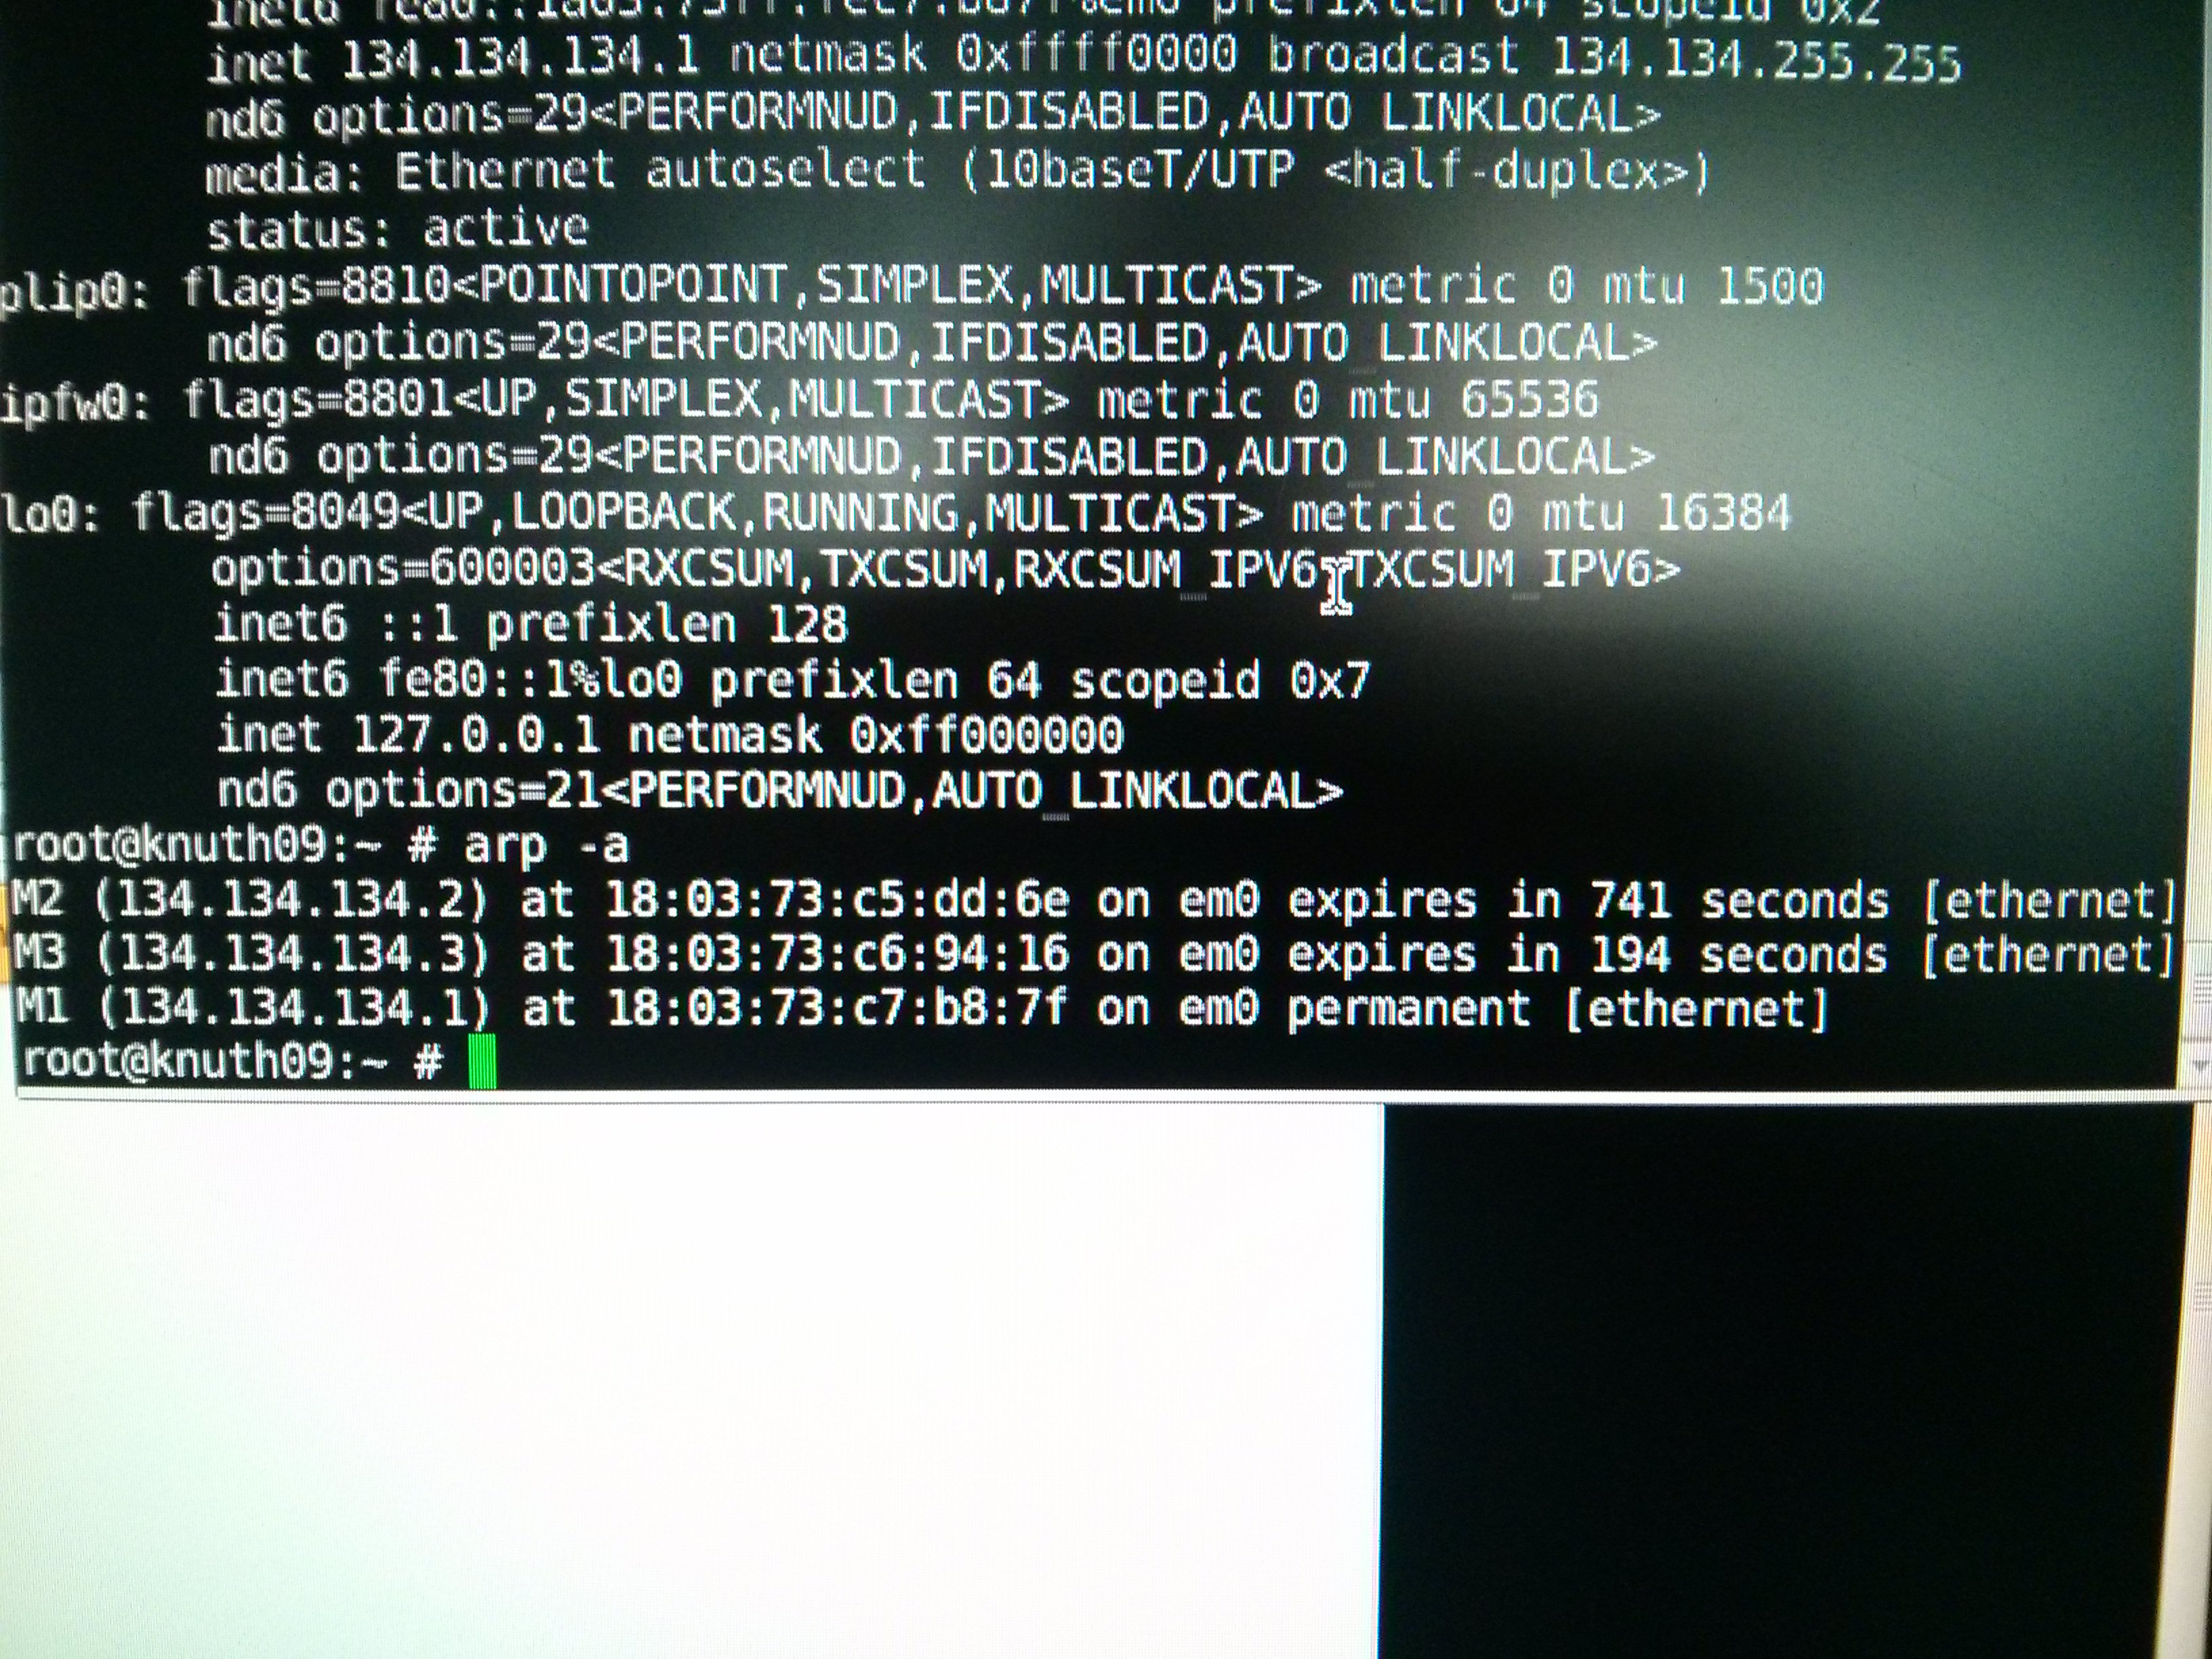
\includegraphics[width=10cm]{screen7.jpg}

\end{itemize}

\section*{2.3	Observation du protocole CSMA/CD}

\begin{itemize}\renewcommand{\labelitemi}{$\bullet$}
\item Nous avons exécuté la commande "udpmt -s 2000 -p 55000 192.168.0.4" sur M2 (192.168.0.3) et au préalable nous avions exécuté "udptarget -p 55000" sur la machine d'adresse 192.168.0.4.
\item On remarque qu'il n'y a aucune collision puisque qu'il n'y a qu'une seule machine qui émet vers une autre.
\item En exécutant udpmt sur une troisième à destination d'une quatrième machine, on remarque que des collisions apparaissent dans netstat.
\item Le nombre de collisions augmente au fur et à mesure. 
\item Plus les paquets sont petits, plus on observe de collisions. Plus les paquets sont petits plus la carte réseau envoie un nombre important de paquets augmentant ainsi la probabilité de collisions.
	\begin{itemize}
	\item Le protocole CSMA permet de détecter si le support est libre et ainsi d'émettre que si celui-ci est libre.
	\item Le protocole CD permet de détecter une collision en écoutant le support pendant qu'une machine émet. S'il y a une différence entre ce qu'elle émet et ce que le support reçoit c'est qu'il y a eu une collision.
	\end{itemize}
\item \begin{itemize}
	\item Taille des paquets : 1472 o, Débit : 5617 kb/s\\
\begin{math}T_{emis} = \cfrac{\left(\cfrac{1472*8}{1024}\right)}{5617}\approx 0,00205 s \end{math}\\
$T_{prop}$ = 1.5/1080000 = 1.4 * $10^{-6}$ s
	\end{itemize} 
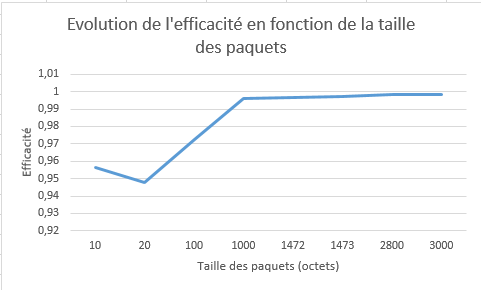
\includegraphics[width=10cm]{efficacite.png}\\
\item On constate qu'à partir d'une certaine taille de paquets (ici à peu près 1000 octets) l'efficacité augmente peu et reste assez stable.
\end{itemize}


\section*{2.4 Analyse des performances du réseau}
\subsection*{2.4.1 Mesure du débit applicatif}

\begin{tabular}{|p{2cm}|p{1cm}|p{1cm}|p{1cm}|p{1cm}|p{1cm}|p{1cm}|p{1cm}|p{1cm}|}

\hline
Taille des paquets (en octets) & 10 & 20 & 100 & 1000 & 1472 & 1473 & 2800 & 3000 \\
\hline
Débit physique (kb/s) & 477 & 1145 & 2945 & 4339 & 5617 & 4733 & 4595 & 4604 \\
\hline
Débit applicatif théorique<= à (kb/s) & 74 \[(477*\]\[\frac{10}{64})\] & 309,5 & 1912,3 & 4116,7 & 5418,2 & 4565,6 & 4508,1 & 4522,6 \\
\hline
\end{tabular}

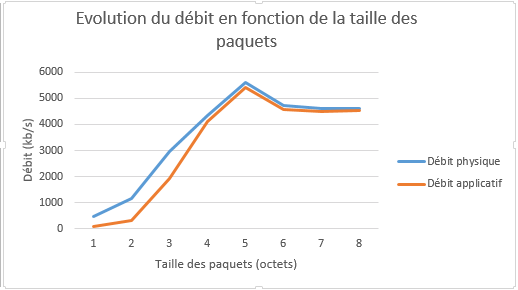
\includegraphics[width=12cm]{debit.png}\\

\paragraph{}Plus la taille des données augmente, plus le débit applicatif approche du débit physique.


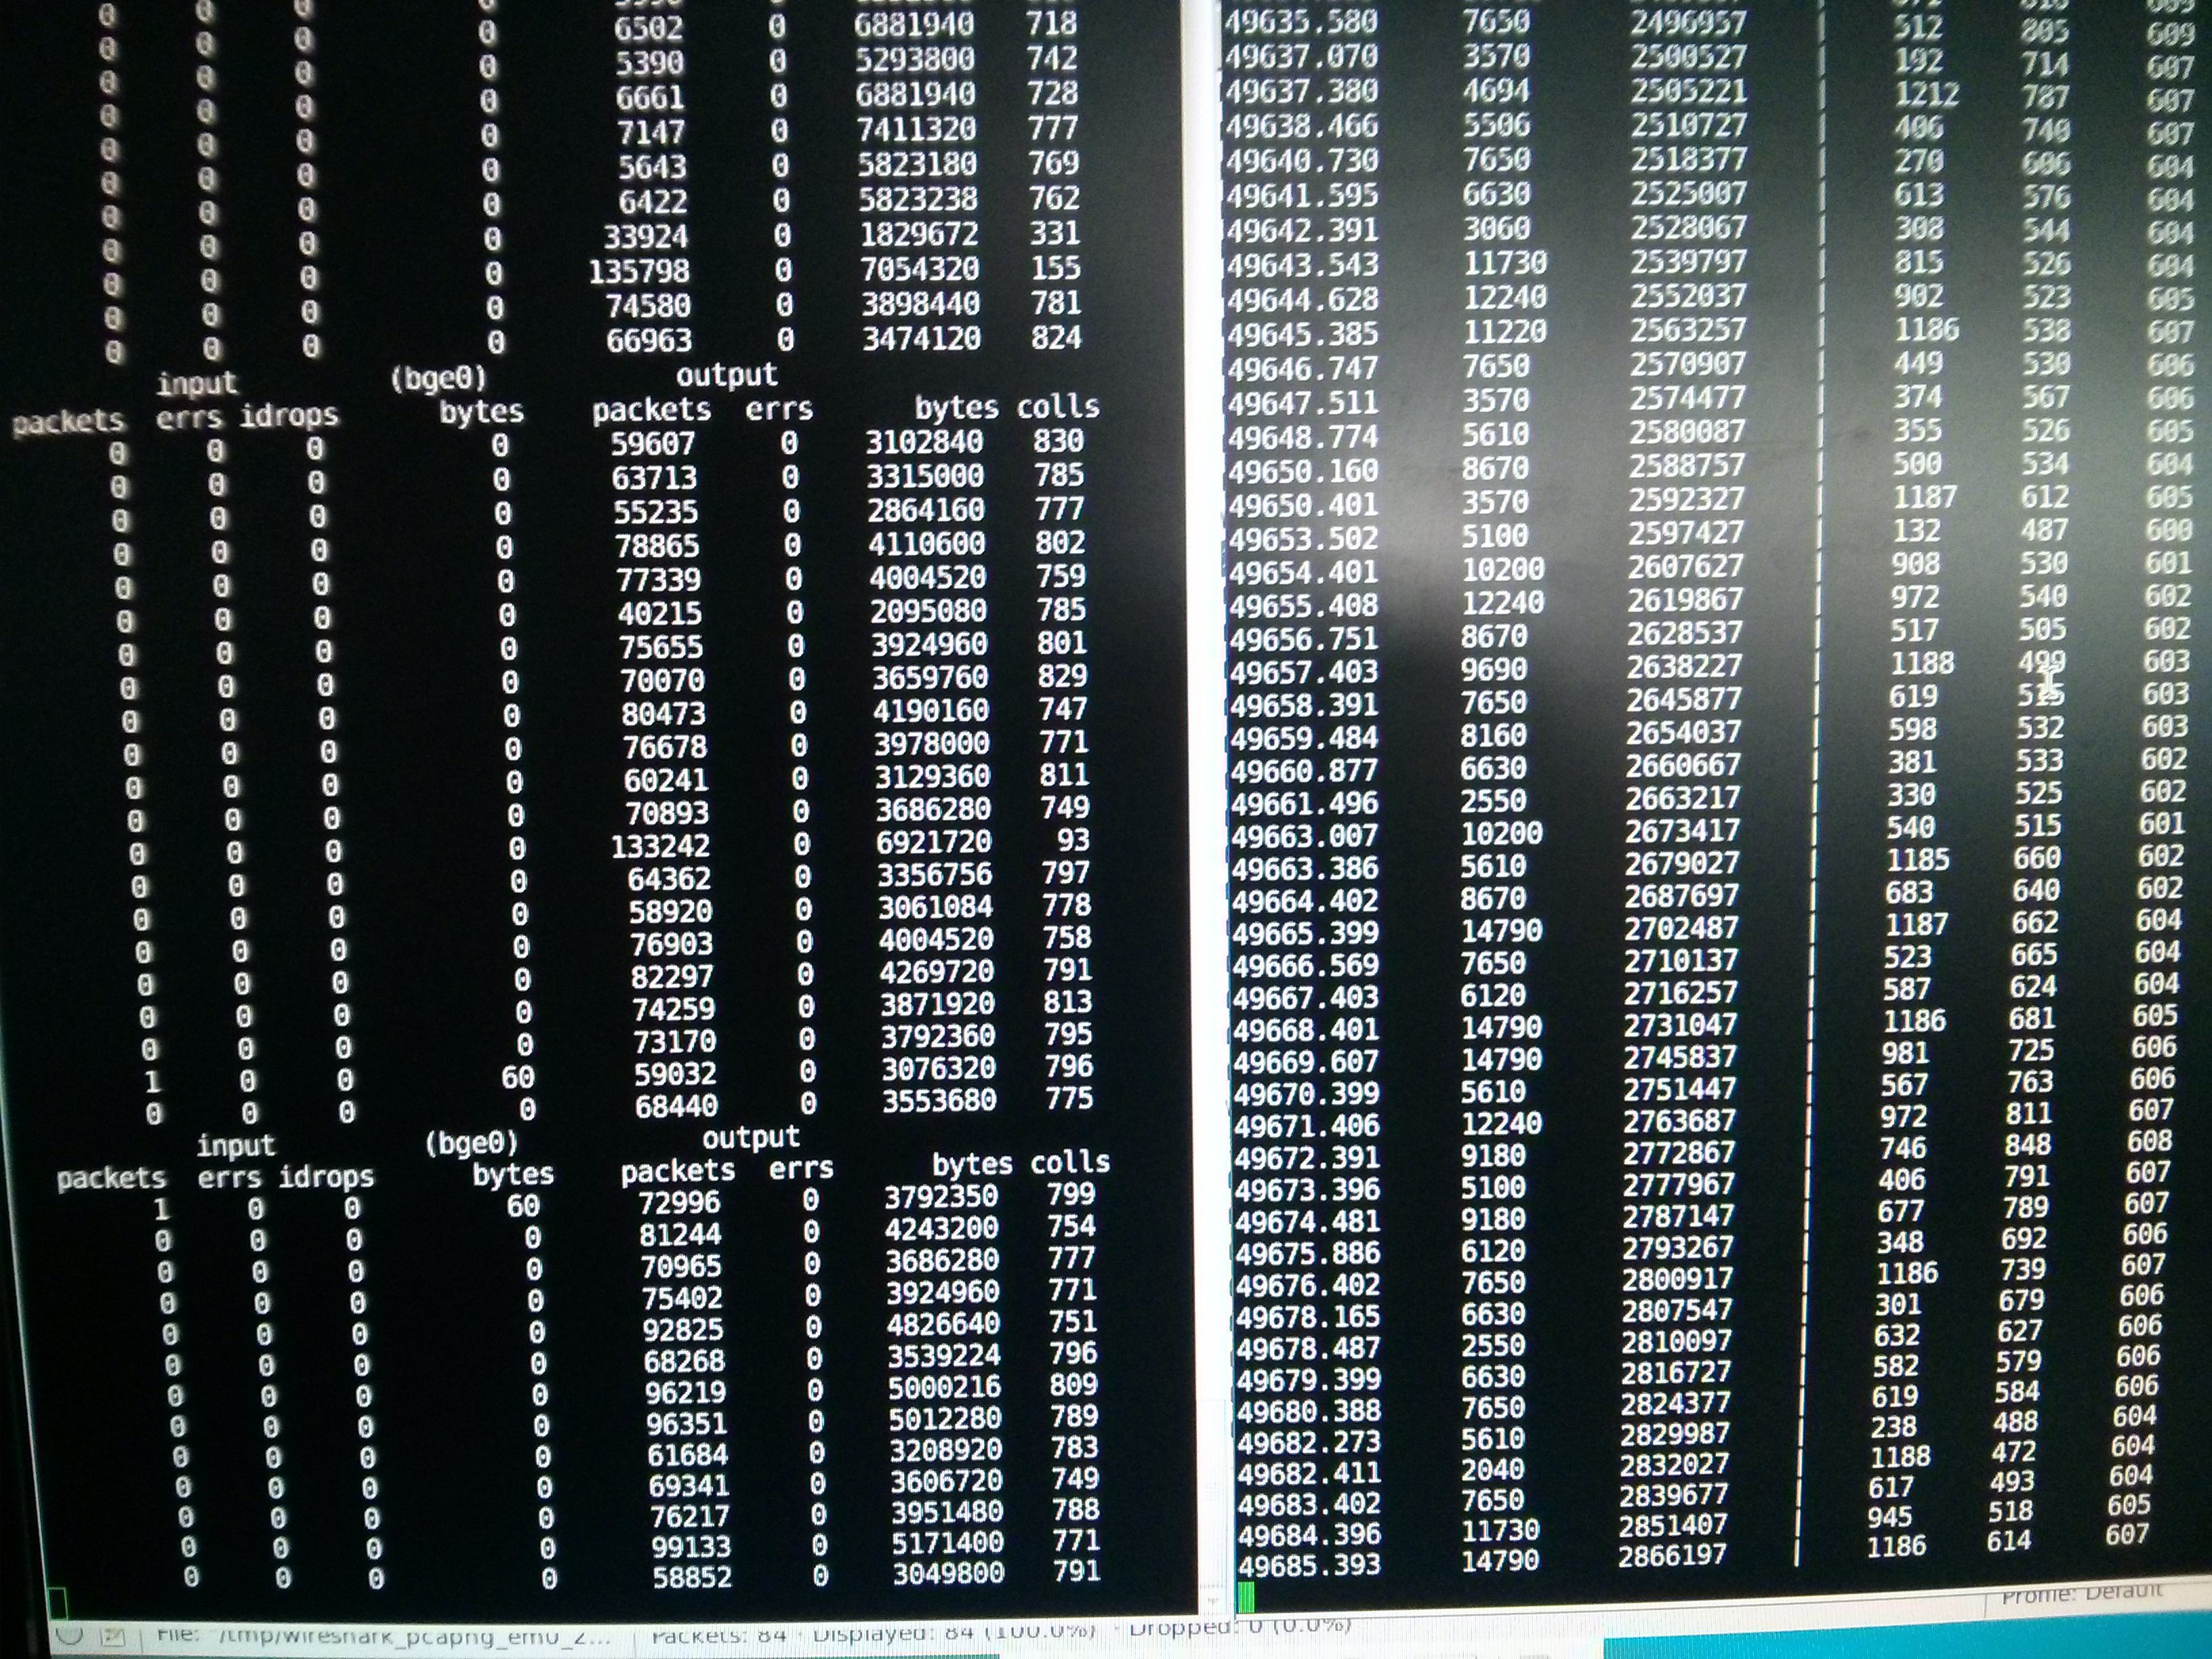
\includegraphics[width=12cm]{screen8.jpg}\\

\subsection*{2.4.2 Mesure de latence}
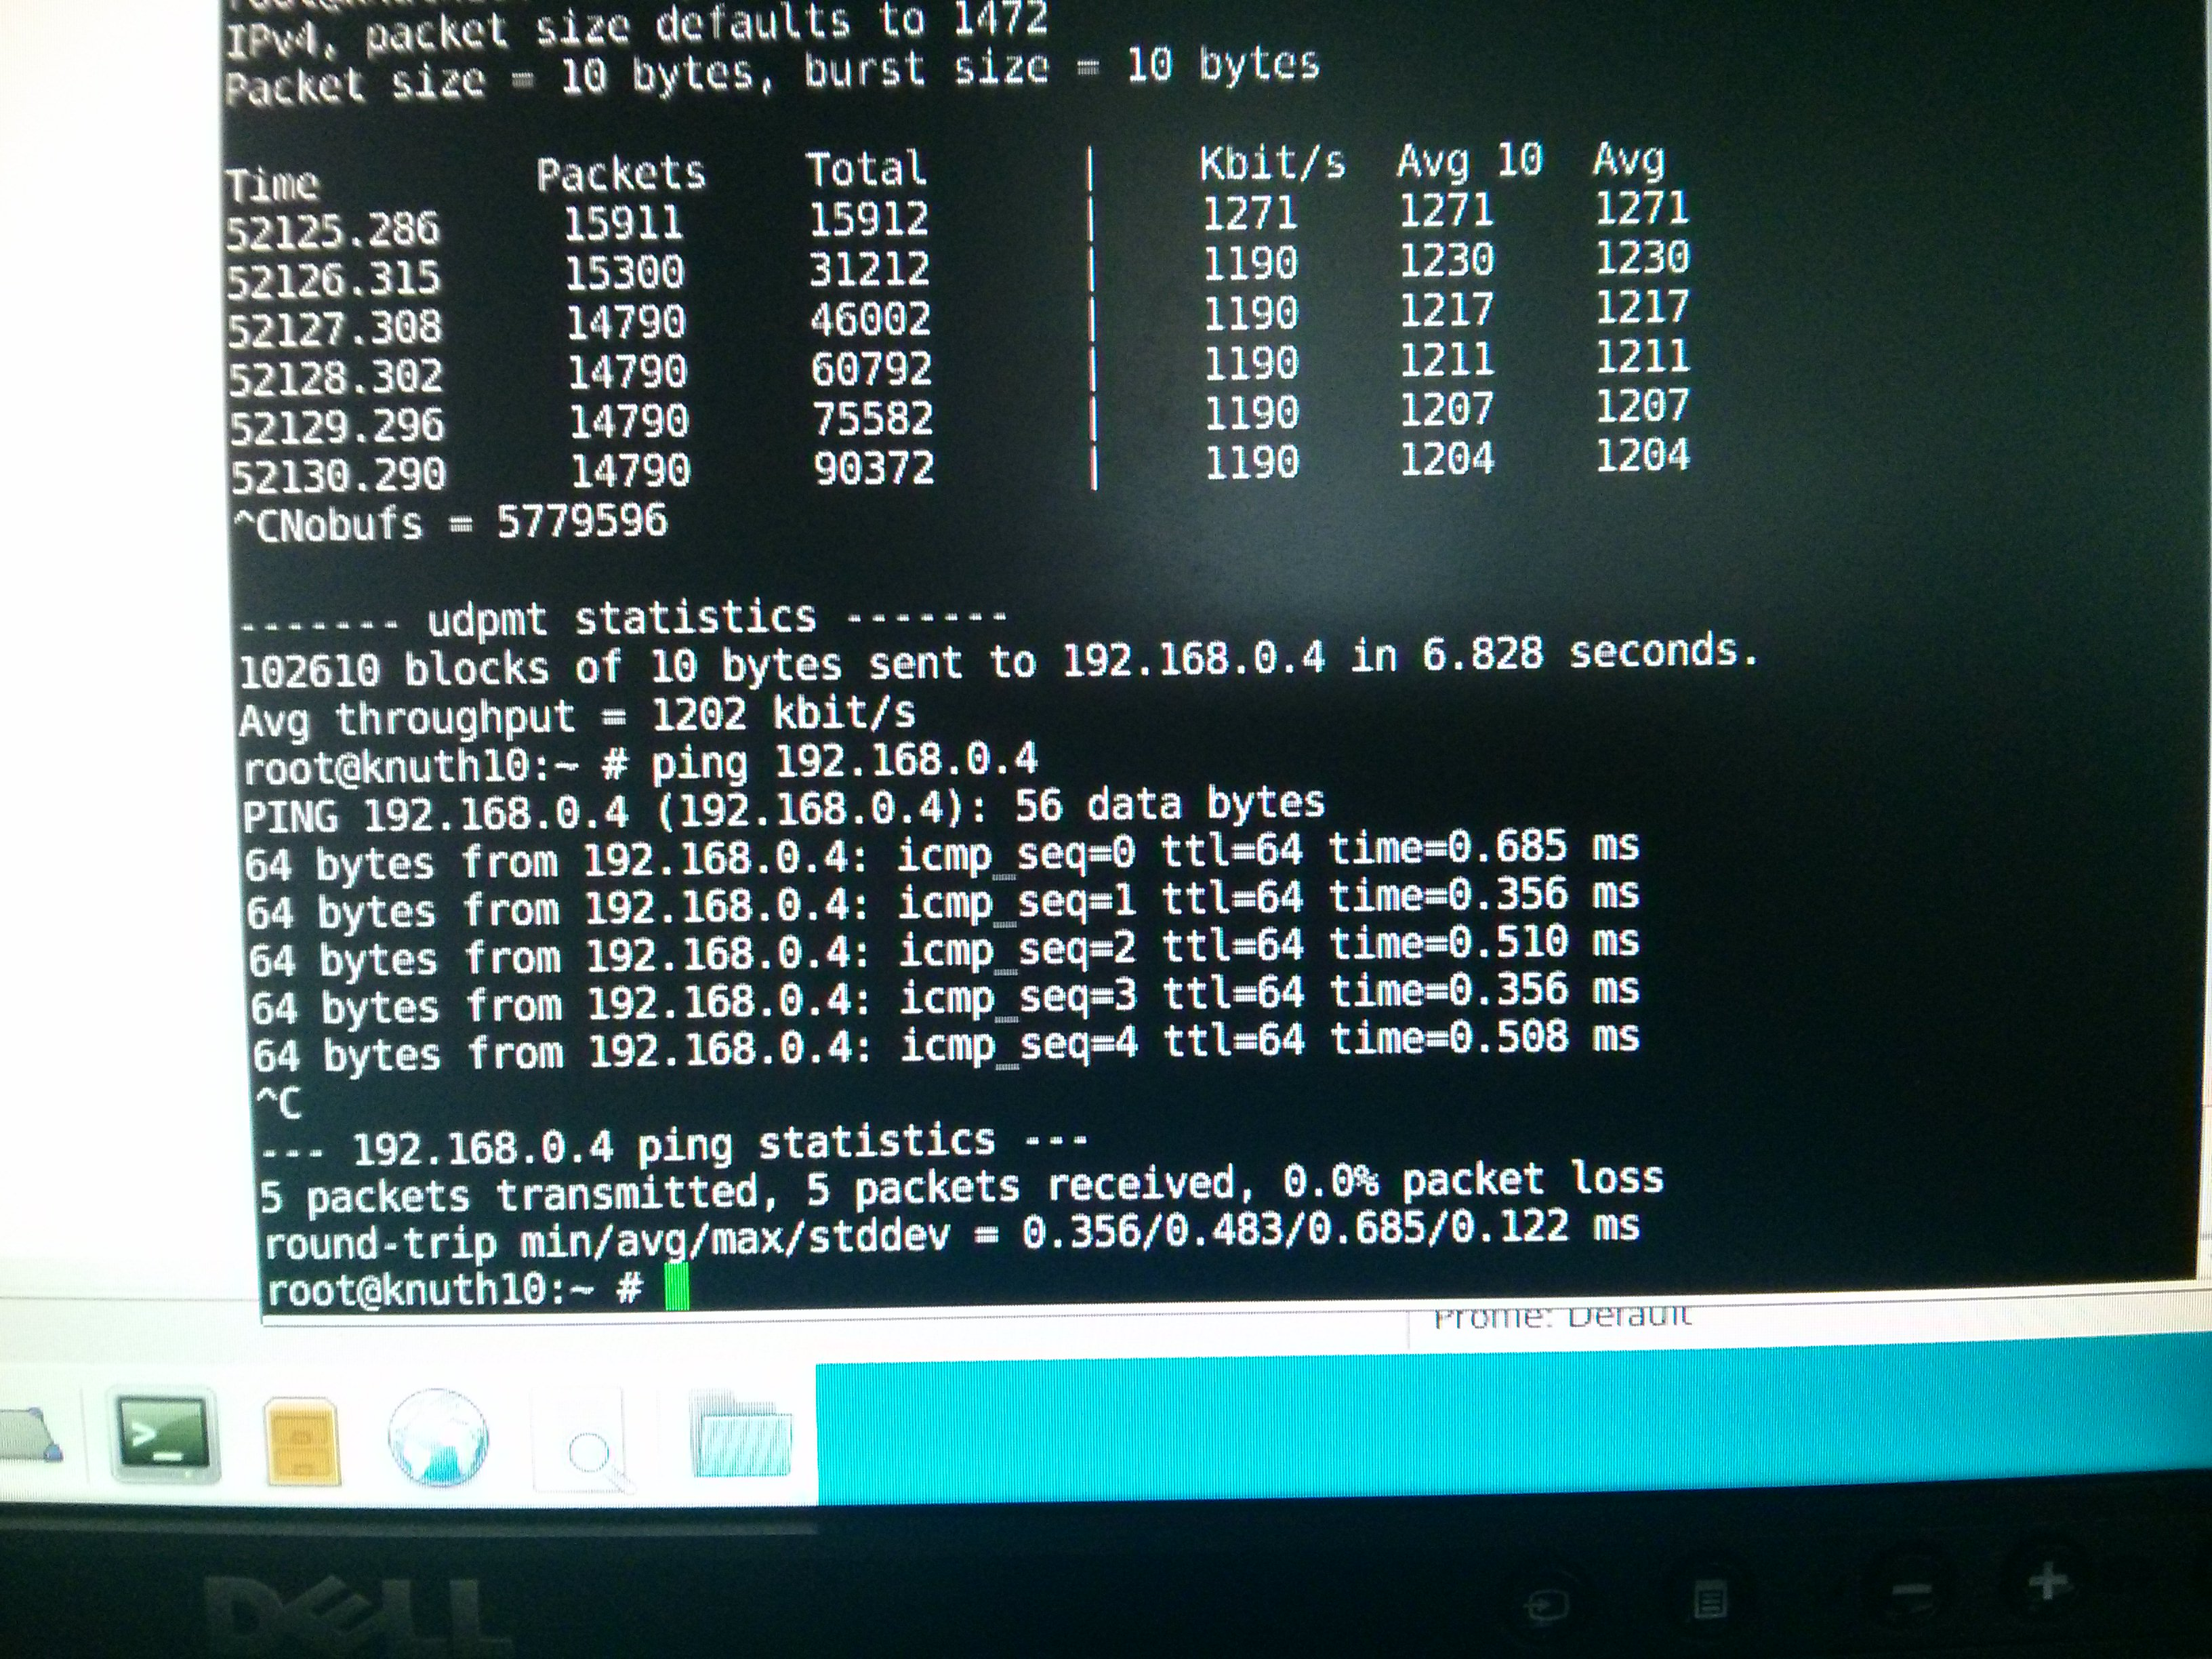
\includegraphics[width=10cm]{screen9.jpg}\\
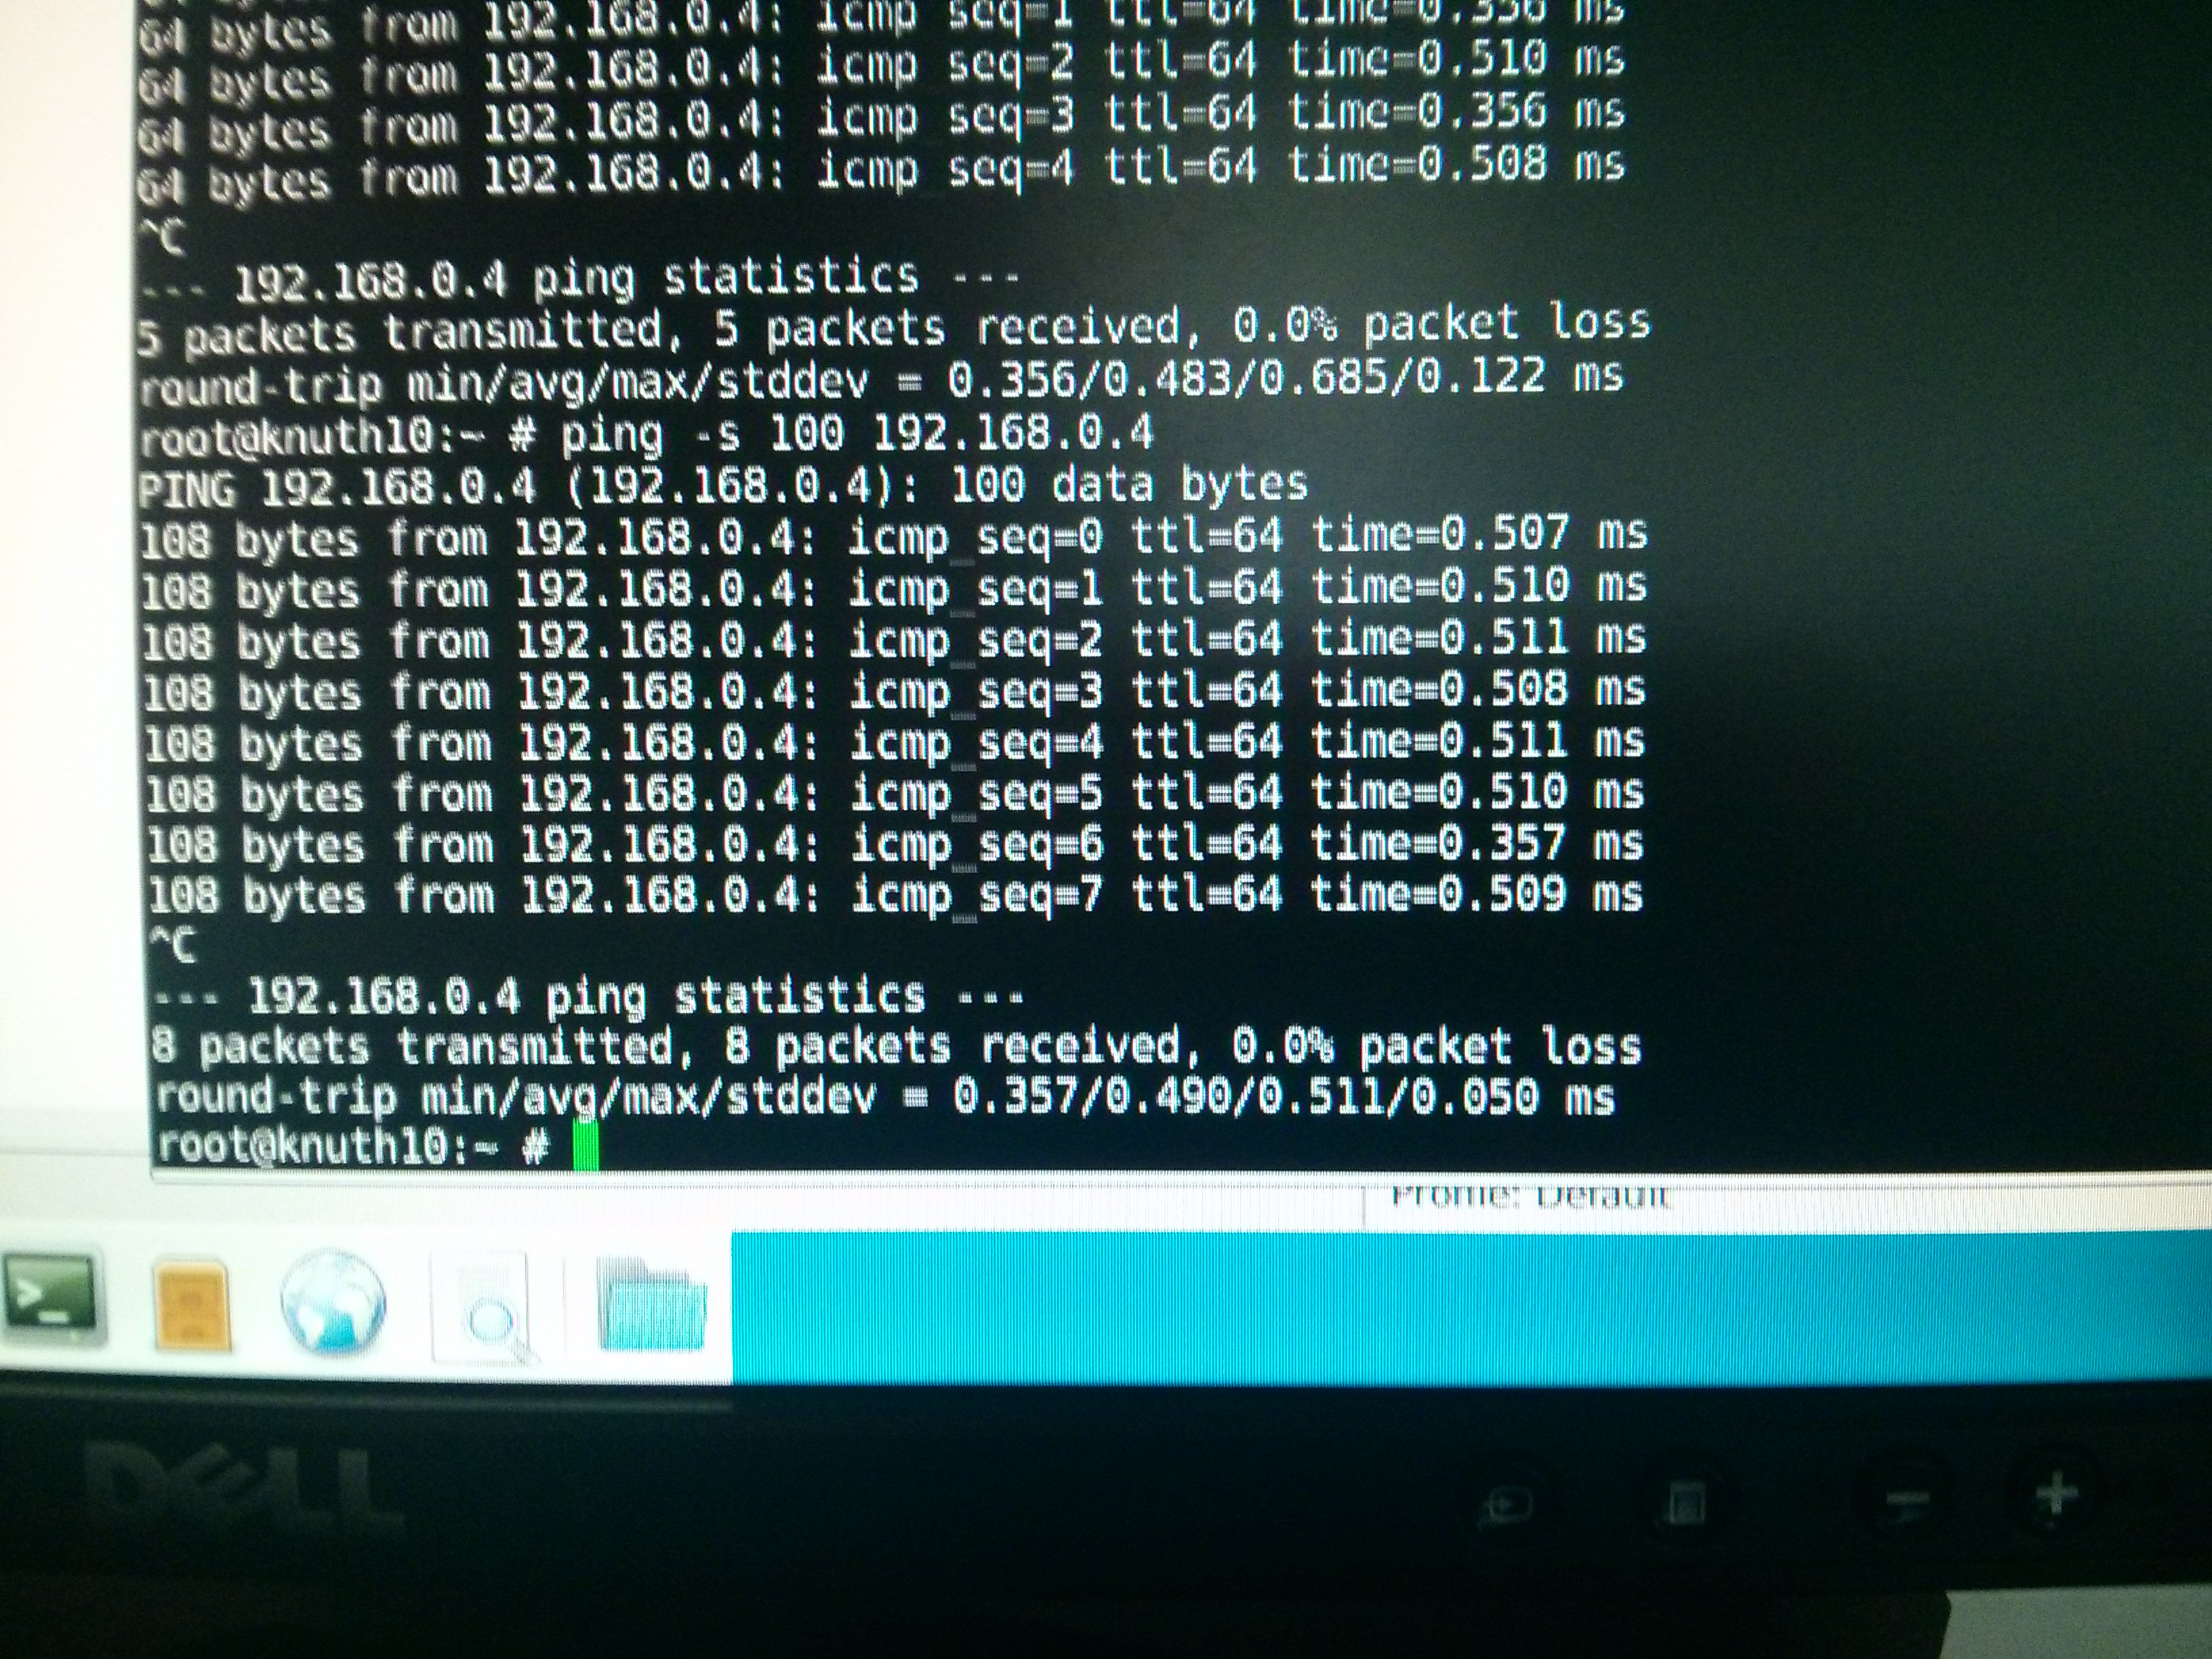
\includegraphics[width=10cm]{screen10.jpg}

\end{document}